\documentclass[11pt]{article}

\usepackage[a4paper,margin=1in]{geometry}
\usepackage[T1]{fontenc}
\usepackage[utf8]{inputenc}
\usepackage{lmodern}
\usepackage{microtype}
\usepackage{amsmath,amssymb,amsthm,mathtools}
\usepackage{booktabs}
\usepackage{graphicx}
\usepackage{float}
\usepackage{placeins}
\usepackage{enumitem}
\usepackage[numbers,sort&compress]{natbib}
\usepackage{xcolor}
\usepackage{xurl}
\usepackage[colorlinks=true,linkcolor=blue!55!black,citecolor=blue!55!black,urlcolor=blue!55!black]{hyperref}
\usepackage[nameinlink,noabbrev]{cleveref}

\setlength{\parindent}{1.4em}
\setlength{\parskip}{0.15em}
\setlist{itemsep=0.25em,topsep=0.35em}

\newtheorem{theorem}{Theorem}[section]
\newtheorem{proposition}[theorem]{Proposition}
\newtheorem{lemma}[theorem]{Lemma}
\newtheorem{corollary}[theorem]{Corollary}
\theoremstyle{definition}
\newtheorem{definition}[theorem]{Definition}
\newtheorem{assumption}[theorem]{Assumption}
\theoremstyle{remark}
\newtheorem{remark}[theorem]{Remark}
\crefname{assumption}{Assumption}{Assumptions}
\Crefname{assumption}{Assumption}{Assumptions}

\newcommand{\R}{\mathbb R}
\newcommand{\C}{\mathbb C}
\newcommand{\N}{\mathbb N}
\newcommand{\uc}{u_{\mathrm c}}
\newcommand{\cK}{\mathcal K}
\newcommand{\cL}{\mathcal L}
\newcommand{\Id}{\operatorname{Id}}
\newcommand{\tr}{\operatorname{tr}}
\newcommand{\spec}{\operatorname{spec}}
\newcommand{\dist}{\operatorname{dist}}
\newcommand{\one}{\mathbf 1}
\newcommand{\Det}{\operatorname{det}}

\title{\textbf{Parity-Renormalized Long-Cycle Determinants}\
\textbf{at a Quadratic Band-Merging Map:}\\
\large Exact Markov Counts, Noncommuting Small-Noise Limits,\
and a Logarithmic Cycle Horizon}
\author{Liang Wang\\
\small School of Artificial Intelligence and Automation,\\[-0.2em]
\small Huazhong University of Science and Technology, Wuhan 430074, P.R. China\\
\small \texttt{wangliang.f@gmail.com}}
\date{July 2026}

\begin{document}

\maketitle

\begin{abstract}
Fixed-length small-noise localization turns a Gaussian cycle trace into a
deterministic periodic-orbit sum, but it gives no uniform control when the
cycle length grows.  We identify the first exact obstruction at the algebraic
band-merging parameter of the quadratic family $f_u(x)=1-u x^2$.

Let $\uc$ be the root in $(1,2)$ of
$u^3-2u^2+2u-2=0$, put $r=\uc-1$, and set
$\lambda=2\uc r=1.678573510428\ldots$.  The three-state Markov graph gives the
exact number of distinct real roots of $f_{\uc}^m(x)=x$:
\[
 N_m=\begin{cases}
 1,&m\ \text{odd},\\
 2^{m/2+1}-1,&m\ \text{even}.
 \end{cases}
\]
The subtraction is a genuine boundary-coding multiplicity, not a numerical
correction.  For every even $m$ we construct a primitive cycle with itinerary
$CA(CB)^{m/2-1}$ and prove
\[
 1-p_m\sim C_*\lambda^{-m},\qquad C_*>0.
\]
Therefore any uniform use of the interior Gaussian localization theorem can
reach at most
$m=(\log(1/\sigma))/\log\lambda+O(1)$.  This logarithmic cycle horizon is an
unconditional consequence of the exact inverse branches.

Write
$P_m=\sum_{f_{\uc}^m(x)=x}|1-(f_{\uc}^m)'(x)|^{-1}$.  Odd lengths satisfy the
exact identity $P_m=(1+\lambda^m)^{-1}$.  Under a separately stated adapted
flat-trace gap hypothesis, $P_m=1+(-1)^m+O(\theta^m)$ for some $\theta<1$.
For every fixed $\sigma>0$, by contrast, the normalized Gaussian operator is
strongly positive and compact, its square is trace class, and
$\tr\cK_\sigma^m\to1$.  Fixed-length localization then yields the conditional
but rigorous noncommutation
\[
 \lim_{\sigma\downarrow0}\lim_{k\to\infty}\tr\cK_\sigma^{2k}=1,
 \qquad
 \lim_{k\to\infty}\lim_{\sigma\downarrow0}\tr\cK_\sigma^{2k}=2.
\]

The correct Hilbert--Schmidt determinant removes both the Perron mode and the
negative parity mode.  At zero noise their exact factor is $1-z^2$.
Dense folded computations through dimension $2560$ verify all finite
identities.  They give
$1+\lambda_-(\sigma)\asymp\sigma^{0.667416}$ on the five smallest resolved
noise levels and show a parity lifetime much longer than the logarithmic
localization horizon.  The exponent $2/3$, the observed even centered-trace
rate, and convergence of the negative resonance to $-1$ are reported as
numerical evidence, not as theorems.
\end{abstract}

\noindent\textbf{Keywords:} quadratic map; band merging; periodic-orbit
trace; small-noise limit; regularized determinant; parity resonance; Markov
partition.

\medskip
\noindent\textbf{MSC 2020:} 37E05; 37C30; 47B10; 47A10; 60J05.

\section{Introduction}

A trace formula at one fixed cycle length and a determinant assembled from
all cycle lengths are different mathematical statements.  For the normalized
Gaussian perturbation of a deterministic map, every fixed positive noise
produces a compact operator.  In the zero-noise limit the kernel concentrates
on a graph, and periodic orbits replace smooth spectral data.  Even if every
fixed trace has a limit, exchanging that limit with an infinite trace series
requires uniform information in the cycle length.

The preceding fixed-length result for Gaussian quadratic Markov cocycles
proved, under interiority and nondegeneracy of the deterministic cycles, that
for each fixed $m\ge2$,
\begin{equation}\label{eq:fixed-length-recalled}
 \tr\cK_\sigma^m
 =\sum_{f^m(x)=x}\frac{1}{|1-(f^m)'(x)|}+O_m(\sigma^2).
\end{equation}
The proof also isolated boundary contact, multiplier one, and deterioration
of the off-orbit action gap as the exact possible sources of nonuniformity
\citep{WangSmallNoise2026}.  The present paper studies the first of these
sources at a parameter where the symbolic geometry is completely explicit.

The parameter is the first algebraic band-merging value of
$f_u(x)=1-u x^2$.  Its invariant core has a period-two decomposition and a
three-state Markov matrix with eigenvalues $0,\sqrt2,-\sqrt2$.  The exact
geometry and the associated $-1$ peripheral mode were established in
\citet{WangParity2026}.  Here the same partition is used for a different
purpose: exact physical periodic-point counts, boundary crowding, long-cycle
trace limits, and regularized determinants.

There are two reasons to separate parity before taking any long-cycle limit.
First, the deterministic system exchanges two components, so its formal
peripheral trace is $1+(-1)^m$.  Second, every fixed positive Gaussian width
destroys the exact decomposition: strong positivity leaves only the Perron
eigenvalue on the unit circle.  Thus the negative mode is long-lived but not
permanent.  The corresponding limits need not commute.

Periodic-orbit determinants and transfer-operator traces are classical for
expanding and piecewise monotone systems
\citep{Ruelle1976,BaladiKeller1990,Baladi2000,Baladi2018}.  The critical map
used here is postcritically finite but not uniformly expanding in its original
interval coordinate.  Correlation decay on its two mixing components follows
from standard Misiurewicz-map theory
\citep{Misiurewicz1981,Young1992,deMeloVanStrien1993}; however, an ordinary
correlation gap does not by itself identify a flat trace of every power.
Rather than silently equating these statements, we place the needed
flat-trace estimate in an explicit hypothesis.  All Markov counting, boundary
crowding, fixed-noise return to the Perron trace, and determinant algebra are
proved independently of that hypothesis.

\subsection*{Main results and logical status}

The conclusions are deliberately divided into three levels.
\begin{enumerate}[label=\textbf{R\arabic*.},leftmargin=3.2em]
 \item \textbf{Exact and unconditional.}  The physical fixed-point count is
 $1$ at odd length and $2^{m/2+1}-1$ at even length.  At odd length the only
 point is $r=\uc-1$, giving $P_m=(1+\lambda^m)^{-1}$.

 \item \textbf{Exact and unconditional.}  A primitive even cycle approaches
 the upper boundary at rate $C_*\lambda^{-m}$.  Hence the interiority input in
 \eqref{eq:fixed-length-recalled} has a logarithmic, not algebraic, uniform
 cycle horizon.

 \item \textbf{Exact and unconditional.}  For fixed $\sigma>0$,
 $\tr\cK_\sigma^m\to1$ exponentially in $m$.  This follows from strong
 positivity, compactness, and the Hilbert--Schmidt eigenvalue bound.

 \item \textbf{Conditional theorem.}  Under the adapted flat-trace gap
 \cref{ass:flat-trace-gap}, $P_{2k}\to2$.  Together with fixed-length
 localization, this proves that the two iterated limits are $1$ and $2$.

 \item \textbf{Exact determinant algebra.}  Subtracting $1+(-1)^m$ from the
 deterministic coefficients removes the factor $1-z^2$.  At finite noise,
 subtracting $1+\lambda_-(\sigma)^m$ removes the actual Perron and parity
 resonances from the Hilbert--Schmidt regularized determinant.

 \item \textbf{Numerical evidence.}  The distinguished negative resonance
 has a gap consistent with $\sigma^{2/3}$, while the even deterministic
 centered traces are consistent with $\lambda^{-m/2}$.  Neither rate is used
 in an unconditional theorem.
\end{enumerate}

The result is a long-cycle audit of the Gaussian dynamical construction.  It
does not identify the negative resonance with a self-adjoint eigenvalue, and
it does not promote coefficientwise small-noise convergence to convergence of
an unrenormalized infinite determinant.

\section{Algebraic band-merging geometry}
\label{sec:geometry}

Let
\begin{equation}\label{eq:family}
 f_u(x)=1-u x^2,
 \qquad I=[-1,1].
\end{equation}
Let $\uc$ be the unique root in $(1,2)$ of
\begin{equation}\label{eq:parameter-polynomial}
 u^3-2u^2+2u-2=0,
\end{equation}
and define
\begin{equation}\label{eq:r-lambda}
 r=\uc-1,
 \qquad
 \lambda=2\uc r.
\end{equation}
Numerically,
\begin{equation}\label{eq:constants-numerical}
 \uc=1.543689012692075\ldots,
 \quad r=0.543689012692075\ldots,
 \quad \lambda=1.678573510428318\ldots.
\end{equation}

The polynomial in \eqref{eq:parameter-polynomial} is strictly increasing on
$(1,2)$ and changes sign there.  Its defining identity gives
\begin{equation}\label{eq:critical-orbit}
 0\longmapsto1\longmapsto-r\longmapsto r\longmapsto r.
\end{equation}
In particular, $X=[-r,1]=f_{\uc}(I)$ is forward invariant, and every periodic
point in $I$ belongs to $X$.

Put
\begin{equation}\label{eq:partition}
 A=[-r,0],\qquad B=[0,r],\qquad C=[r,1].
\end{equation}
Up to common endpoints,
\begin{equation}\label{eq:images}
 f(A)=C,\qquad f(B)=C,\qquad f(C)=A\cup B,
\end{equation}
where $f=f_{\uc}$.  Thus the transition matrix is
\begin{equation}\label{eq:markov-matrix}
 M=
 \begin{pmatrix}
 0&0&1\\
 0&0&1\\
 1&1&0
 \end{pmatrix},
 \qquad
 \spec(M)=\{0,\sqrt2,-\sqrt2\}.
\end{equation}
The graph is bipartite: $A,B$ form one side and $C$ the other.

\subsection{Exact symbolic and physical counts}

Let
\begin{equation}\label{eq:Nm-definition}
 N_m=\#\{x\in I:f^m(x)=x\}
\end{equation}
count distinct real points, without multiplicity.

\begin{theorem}[Exact physical fixed-point count]
\label{thm:exact-count}
For every $m\ge1$,
\begin{equation}\label{eq:exact-count}
 N_m=
 \begin{cases}
 1,&m\text{ odd},\\[0.2em]
 2^{m/2+1}-1,&m\text{ even}.
 \end{cases}
\end{equation}
All these fixed points are simple.
\end{theorem}

\begin{proof}
The critical orbit \eqref{eq:critical-orbit} is finite and lands on the
repelling fixed point $r$, whose multiplier is $f'(r)=-\lambda$ with
$\lambda>1$.  Thus $f$ is a postcritically finite Misiurewicz map.  Standard
Markov coding supplies one closed symbolic path for each periodic point not
on a partition boundary, and one periodic point for each such path; there are
no homtervals, and every periodic orbit is repelling
\citep{deMeloVanStrien1993,Baladi2000}.  The only periodic partition endpoint
is $r$: the remaining endpoints enter its orbit by
\eqref{eq:critical-orbit}.

The number of length-$m$ closed paths with a marked initial state is
\begin{equation}\label{eq:symbolic-count}
 \tr M^m=
 \begin{cases}
 0,&m\text{ odd},\\
 2^{m/2+1},&m\text{ even},
 \end{cases}
\end{equation}
by \eqref{eq:markov-matrix}.  For even $m=2k$, the physical fixed point $r$
has the two alternating boundary codes $(BC)^k$ and $(CB)^k$.  Every other
closed path codes a distinct interior point.  Hence one must subtract exactly
one from the symbolic count.

For odd $m$ the bipartite graph has no closed path.  Nevertheless the
exceptional boundary point $r$ is fixed and therefore solves $f^m(x)=x$.
There is no other periodic boundary point, so it is the unique solution.
Repulsion excludes multiplier one and proves simplicity.
\end{proof}

The difference between \eqref{eq:symbolic-count} and
\eqref{eq:exact-count} is important.  Treating $\tr M^m$ as a physical root
count would miss the odd fixed point and double-count the even boundary code.

\subsection{Exact odd flat traces}

Define the deterministic flat trace
\begin{equation}\label{eq:flat-trace}
 P_m=\sum_{f^m(x)=x}\frac{1}{|1-(f^m)'(x)|}.
\end{equation}

\begin{corollary}[Odd trace formula]
\label{cor:odd-trace}
For every odd $m\ge1$,
\begin{equation}\label{eq:odd-trace}
 P_m=\frac{1}{1+\lambda^m}.
\end{equation}
In particular, $P_m=O(\lambda^{-m})$ along odd lengths.
\end{corollary}

\begin{proof}
By \cref{thm:exact-count}, the only point is $r$.  Since
$(f^m)'(r)=(-\lambda)^m=-\lambda^m$ for odd $m$, its weight is
$(1+\lambda^m)^{-1}$.
\end{proof}

\section{An explicit boundary cycle and the logarithmic horizon}
\label{sec:boundary}

For $y\in[-r,1]$, the two inverse branches are
\begin{equation}\label{eq:inverse-branches}
 g_+(y)=\sqrt{\frac{1-y}{\uc}},
 \qquad
 g_-(y)=-\sqrt{\frac{1-y}{\uc}}.
\end{equation}
The symbols $B,C$ use $g_+$ and the symbol $A$ uses $g_-$.  Introduce
\begin{equation}\label{eq:hq}
 h=g_+\circ g_+,
 \qquad
 q=g_+\circ g_-.
\end{equation}
At the fixed point $r$,
\begin{equation}\label{eq:hq-data}
 h(r)=r,\qquad h'(r)=\lambda^{-2},\qquad
 q(r)=1,\qquad q'(r)=-\frac{1}{2\uc\lambda}.
\end{equation}

For $m=2k$, consider the closed word
\begin{equation}\label{eq:boundary-word}
 w_{2k}=CA(CB)^{k-1}.
\end{equation}
Its inverse composition is
\begin{equation}\label{eq:boundary-inverse-composition}
 G_{2k}=q\circ h^{k-1}.
\end{equation}

\begin{theorem}[Exponential boundary crowding]
\label{thm:boundary-crowding}
For every $k\ge1$, the word $w_{2k}$ codes a primitive physical periodic
point $p_{2k}\in(r,1)$.  There exists a constant $C_*>0$ such that
\begin{equation}\label{eq:boundary-asymptotic}
 1-p_{2k}\sim C_*\lambda^{-2k}
 \qquad(k\to\infty).
\end{equation}
In particular,
\begin{equation}\label{eq:boundary-theta}
 1-p_m=\Theta(\lambda^{-m})
 \qquad(m\to\infty,\ m\text{ even}).
\end{equation}
\end{theorem}

\begin{proof}
The word \eqref{eq:boundary-word} is an allowed closed path.  Markov coding
therefore gives a unique fixed point of \eqref{eq:boundary-inverse-composition}.
It is not an endpoint because the word contains $A$, and it is primitive
because $A$ occurs exactly once: a nontrivial repeated word would contain at
least two copies of $A$.

The map $h$ is increasing on $(r,1)$, has no fixed point there, and
$h(x)<x$ for $x>r$.  Its iterates converge to $r$, uniformly on compact
subintervals and, after the first iterate, uniformly on $[r,1]$.  Since
$p_{2k}=q(h^{k-1}(p_{2k}))$ and $q(r)=1$, it follows first that
$p_{2k}\to1$.

We record the standard attracting-fixed-point estimate.  Put
$a=h'(r)=\lambda^{-2}$.  Linearization of the $C^2$ map $h$ near $r$ gives a
strictly increasing coordinate $\psi$ on its basin such that
\begin{equation}\label{eq:koenigs}
 \psi(h(x))=a\psi(x),\qquad
 \psi(r)=0,\qquad \psi'(r)=1.
\end{equation}
Although $h'$ is singular at the endpoint $1$, one iterate sends a
neighborhood of $1$ into a compact interior interval.  Thus
$\psi(1):=a^{-1}\psi(h(1))$ is finite and positive, and the same formula
extends $\psi$ continuously near $1$.  Consequently, as $n\to\infty$,
uniformly for $x$ in that neighborhood,
\begin{equation}\label{eq:h-asymptotic}
 h^n(x)-r=a^n\psi(x)(1+o(1)).
\end{equation}
Taylor expansion of $q$ at $r$, followed by
\eqref{eq:h-asymptotic} with $n=k-1$, yields
\begin{align}
 1-p_{2k}
 &=-q'(r)\bigl(h^{k-1}(p_{2k})-r\bigr)(1+o(1))\notag\\
 &=-q'(r)\psi(1)\lambda^{-2(k-1)}(1+o(1))\notag\\
 &=C_*\lambda^{-2k}(1+o(1)),
 \label{eq:boundary-proof-asymptotic}
\end{align}
where $C_*=-q'(r)\psi(1)\lambda^2>0$.
\end{proof}

The numerical value approached by
$(1-p_m)\lambda^m$ is $0.4608\ldots$, but no numerical value of $C_*$ is
needed below.

\subsection{Consequence for small-noise localization}

Let $\Delta_m$ be the smallest distance to $\partial I=\{-1,1\}$ attained by
any point on any cycle satisfying $f^m(x)=x$.  The cycle in
\cref{thm:boundary-crowding} gives
\begin{equation}\label{eq:delta-upper}
 \Delta_{2k}\le1-p_{2k}\le C\lambda^{-2k}
\end{equation}
for all sufficiently large $k$.

The fixed-length proof recalled in \eqref{eq:fixed-length-recalled} replaces a
truncated row normalizer by a full Gaussian normalizer inside each orbit tube.
For a cycle of clearance $\Delta_m$, that step requires at least
$\sigma\ll\Delta_m$; its tail error contains
$\exp[-\Delta_m^2/(C\sigma^2)]$.

\begin{corollary}[Logarithmic localization horizon]
\label{cor:log-horizon}
Suppose a family of cycle lengths $m=m(\sigma)$ includes every deterministic
cycle of that length and is required to satisfy a uniform interior condition
$\Delta_m\ge c\sigma$.  Necessarily,
\begin{equation}\label{eq:horizon-weak}
 m(\sigma)\le
 \frac{\log(1/\sigma)}{\log\lambda}+O(1).
\end{equation}
If the stronger asymptotic condition
$\Delta_m/\sigma\to\infty$ is required, then necessarily
\begin{equation}\label{eq:horizon-strong}
 \log(1/\sigma)-m(\sigma)\log\lambda\longrightarrow+\infty.
\end{equation}
\end{corollary}

\begin{proof}
Combine the lower requirement on $\Delta_m$ with the upper bound
\eqref{eq:delta-upper}, take logarithms, and absorb fixed constants into the
$O(1)$ term.  The same calculation with
$\Delta_m/\sigma\to\infty$ gives \eqref{eq:horizon-strong}.
\end{proof}

\begin{remark}[What the horizon does and does not prove]
The corollary is a rigorous obstruction to applying the existing local
Gaussian proof uniformly beyond logarithmic length.  It does not prove that
the actual noisy trace must fail there; a different boundary-layer analysis
could in principle continue farther.  Such an analysis would have to replace,
not merely reuse, the full-Gaussian orbit formula.
\end{remark}

\section{Deterministic parity centering}
\label{sec:deterministic-centering}

The Markov graph and the component exchange suggest the baseline
\begin{equation}\label{eq:parity-baseline}
 b_m=1+(-1)^m.
\end{equation}
Define centered deterministic coefficients
\begin{equation}\label{eq:centered-coefficients}
 c_m=P_m-b_m.
\end{equation}
By \cref{cor:odd-trace}, $c_m=(1+\lambda^m)^{-1}$ for odd $m$.  The even
asymptotic requires more than topological counting.

\begin{assumption}[Adapted flat-trace gap]
\label{ass:flat-trace-gap}
There are constants $C_0>0$ and $0<\theta<1$ such that
\begin{equation}\label{eq:flat-trace-gap}
 |P_m-1-(-1)^m|\le C_0\theta^m
 \qquad(m\ge1).
\end{equation}
\end{assumption}

This is intentionally stated at the exact strength used below.  A standard
route would construct an adapted tower or weighted inverse-branch space on
the two mixing components of $f^2$, realize $P_m$ as a flat trace, and prove
that the remainder after the two peripheral projectors is flat-trace
summable.  Piecewise-monotone zeta and transfer-operator theory provides the
relevant framework \citep{BaladiKeller1990,Baladi2000,Baladi2018}.  The
ordinary component correlation gap established for this Misiurewicz map does
not, by itself, verify every part of that construction; hence
\cref{ass:flat-trace-gap} is not declared unconditional here.

\begin{proposition}[Conditional deterministic long-cycle limit]
\label{prop:deterministic-limit}
Under \cref{ass:flat-trace-gap},
\begin{equation}\label{eq:deterministic-parity-limit}
 P_{2k}=2+O(\theta^{2k}),
 \qquad
 P_{2k+1}=O(\lambda^{-(2k+1)}).
\end{equation}
In particular, $P_{2k}\to2$ and $P_{2k+1}\to0$.
\end{proposition}

\begin{proof}
The even assertion is \eqref{eq:flat-trace-gap}; the odd assertion follows
unconditionally from \eqref{eq:odd-trace}.
\end{proof}

The direct computations in \cref{sec:numerics} give
$P_{28}=1.9985818867$ and an even centered decay consistent with
$\lambda^{-m/2}$.  Those values support \cref{ass:flat-trace-gap} but do not
replace its functional-analytic proof.

\section{Fixed positive noise and noncommuting limits}
\label{sec:noncommuting}

For $\sigma>0$, define
\begin{align}
 w_\sigma(x,y)&=
 \exp\left[-\frac{(y-f(x))^2}{2\sigma^2}\right],\label{eq:gaussian-weight}\\
 Z_\sigma(x)&=\int_Iw_\sigma(x,z)\,dz,\label{eq:normalizer}\\
 q_\sigma(x,y)&=\frac{w_\sigma(x,y)}{Z_\sigma(x)},\label{eq:kernel}\\
 (\cK_\sigma g)(x)&=\int_Iq_\sigma(x,y)g(y)\,dy.
 \label{eq:operator}
\end{align}
The kernel is continuous and strictly positive on $I^2$, and
$\cK_\sigma\one=\one$.

\begin{theorem}[Fixed-noise long-cycle trace]
\label{thm:fixed-noise-trace}
For every fixed $\sigma>0$, $\cK_\sigma$ is Hilbert--Schmidt on $L^2(I)$,
$\cK_\sigma^2$ is trace class, and
\begin{equation}\label{eq:fixed-noise-limit}
 \tr\cK_\sigma^m\longrightarrow1
 \qquad(m\to\infty, m\ge2).
\end{equation}
More precisely, if $r_\sigma<1$ is the spectral radius after removing the
simple eigenvalue $1$, then
\begin{equation}\label{eq:fixed-noise-rate}
 |\tr\cK_\sigma^m-1|
 \le r_\sigma^{m-2}
 \sum_{j\ge2}|\lambda_j(\sigma)|^2,
\end{equation}
where the non-Perron eigenvalues are repeated by algebraic multiplicity.
\end{theorem}

\begin{proof}
Continuity of the kernel on a compact square makes $\cK_\sigma$
Hilbert--Schmidt.  Therefore its square is trace class
\citep{Kress2014,Simon2005}.  On $C(I)$ the operator has norm one, preserves
$\one$, and is strongly positive.  Compact Perron--Frobenius theory therefore
implies that $1$ is algebraically simple and that every other spectral value
has modulus strictly less than one.  Every nonzero $L^2$ eigenfunction is
continuous because it equals a nonzero scalar multiple of its image under the
continuous-kernel operator.  Expanding
$(\cK_\sigma-\lambda)^p g=0$ shows in the same way that every generalized
eigenvector for $\lambda\ne0$ is a finite linear combination of continuous
images $\cK_\sigma^jg$.  Hence the nonzero spectra on $C(I)$ and $L^2(I)$,
including algebraic multiplicities, agree.  Compactness then gives a common
bound $r_\sigma<1$ for the non-Perron spectrum.

The eigenvalues of a Hilbert--Schmidt operator are square summable.  Lidskii's
theorem applied to $\cK_\sigma^m$, $m\ge2$, gives
\begin{equation}\label{eq:lidskii}
 \tr\cK_\sigma^m
 =1+\sum_{j\ge2}\lambda_j(\sigma)^m.
\end{equation}
Taking absolute values and extracting $r_\sigma^{m-2}$ proves
\eqref{eq:fixed-noise-rate} and the limit.
\end{proof}

For every fixed $m\ge2$, all deterministic periodic points are interior to
$I$ and repelling.  The fixed-length localization theorem
\eqref{eq:fixed-length-recalled} therefore applies and gives
\begin{equation}\label{eq:fixed-m-zero-noise}
 \lim_{\sigma\downarrow0}\tr\cK_\sigma^m=P_m.
\end{equation}

\begin{theorem}[Noncommuting small-noise and long-cycle limits]
\label{thm:noncommuting}
The first iterated even-cycle limit is unconditional:
\begin{equation}\label{eq:first-iterated-limit}
 \lim_{\sigma\downarrow0}\lim_{k\to\infty}
 \tr\cK_\sigma^{2k}=1.
\end{equation}
Under \cref{ass:flat-trace-gap}, the opposite iterated limit exists and is
\begin{equation}\label{eq:second-iterated-limit}
 \lim_{k\to\infty}\lim_{\sigma\downarrow0}
 \tr\cK_\sigma^{2k}=2.
\end{equation}
Thus, under that explicit deterministic input, the limits do not commute.
\end{theorem}

\begin{proof}
Equation \eqref{eq:first-iterated-limit} follows immediately from
\cref{thm:fixed-noise-trace}.  For the opposite order, use
\eqref{eq:fixed-m-zero-noise} first and then
\cref{prop:deterministic-limit}.
\end{proof}

The theorem isolates the singularity.  At fixed noise the negative parity
mode lies strictly inside the unit disk and eventually decays.  At zero noise
the two components exchange exactly, so the parity contribution survives at
every even time.  No finite collection of fixed-$m$ limits can decide which
behavior controls a simultaneous limit.

\section{Parity-renormalized Hilbert--Schmidt determinants}
\label{sec:determinants}

Because $\cK_\sigma$ is Hilbert--Schmidt but is not assumed trace class, the
natural determinant is the second regularized determinant
\citep{Simon2005}:
\begin{equation}\label{eq:det2}
 \Det{}_2(\Id-z\cK_\sigma)
 =\prod_j(1-z\lambda_j)e^{z\lambda_j}
 =\exp\left[-\sum_{m\ge2}
 \frac{z^m}{m}\tr\cK_\sigma^m\right]
\end{equation}
in its trace-series disk, followed by analytic continuation of the entire
product.

\subsection{The deterministic parity factor}

Under \cref{ass:flat-trace-gap}, define
\begin{equation}\label{eq:deterministic-bulk-determinant}
 \widehat D_{0,\mathrm{bulk},2}(z)
 =\exp\left[-\sum_{m\ge2}\frac{c_mz^m}{m}\right].
\end{equation}
The series is analytic for $|z|<\theta^{-1}>1$.  The baseline factor is exact:
\begin{align}
 \exp\left[-\sum_{m\ge2}
 \frac{(1+(-1)^m)z^m}{m}\right]
 &=\exp\left[-\sum_{m\ge1}
 \frac{z^m+(-z)^m}{m}\right]\notag\\
 &=1-z^2.
 \label{eq:parity-factor}
\end{align}
The $m=1$ term vanishes, so the Hilbert--Schmidt regularization changes
nothing in \eqref{eq:parity-factor}.  The formal deterministic determinant is
therefore
\begin{equation}\label{eq:deterministic-factorization}
 \widehat D_{0,2}(z)
 =(1-z^2)\widehat D_{0,\mathrm{bulk},2}(z).
\end{equation}

\subsection{Finite-noise extraction}

Suppose a fixed positive-noise operator has a selected simple negative
resonance $\lambda_-(\sigma)$, as in the computations below.  Define
\begin{equation}\label{eq:noisy-centered-traces}
 c_{\sigma,m}
 =\tr\cK_\sigma^m-1-\lambda_-(\sigma)^m.
\end{equation}
Removing the two corresponding factors from \eqref{eq:det2} gives
\begin{align}
 D_{\sigma,\mathrm{bulk},2}(z)
 &=\exp\left[-\sum_{m\ge2}
 \frac{c_{\sigma,m}z^m}{m}\right]\label{eq:noisy-bulk-det-traces}\\
 &=\prod_{\lambda_j\notin\{1,\lambda_-(\sigma)\}}
 (1-z\lambda_j)e^{z\lambda_j},\label{eq:noisy-bulk-det-product}
\end{align}
and the exact factorization
\begin{align}
 \Det{}_2(\Id-z\cK_\sigma)
 ={}&(1-z)e^z
 (1-z\lambda_-(\sigma))e^{z\lambda_-(\sigma)}
 D_{\sigma,\mathrm{bulk},2}(z).
 \label{eq:noisy-factorization}
\end{align}

\begin{proposition}[Coefficientwise conditional bridge]
\label{prop:coefficientwise-bridge}
If $\lambda_-(\sigma)\to-1$ as $\sigma\downarrow0$, then for every fixed
$m\ge2$,
\begin{equation}\label{eq:coefficientwise-bridge}
 c_{\sigma,m}\longrightarrow c_m.
\end{equation}
Consequently every fixed Taylor coefficient of the finite truncations of
$D_{\sigma,\mathrm{bulk},2}$ converges to its deterministic centered
counterpart.
\end{proposition}

\begin{proof}
Combine \eqref{eq:fixed-m-zero-noise},
$\lambda_-(\sigma)^m\to(-1)^m$, and the definitions
\eqref{eq:centered-coefficients} and \eqref{eq:noisy-centered-traces}.
Every coefficient of fixed degree depends on only finitely many traces.
\end{proof}

The hypothesis $\lambda_-(\sigma)\to-1$ is strongly supported numerically but
is not proved here.  More importantly, coefficientwise convergence does not
provide a common summable majorant in $m$.  The logarithmic horizon in
\cref{cor:log-horizon} shows why that missing step is substantive.

\section{Numerical audit}
\label{sec:numerics}

All calculations use the algebraic root of
\eqref{eq:parameter-polynomial}, rather than its printed decimal.  Periodic
points are generated from every allowed closed Markov word and refined as
fixed points of its inverse composition.  Duplicate endpoint codes are
removed numerically only after the exact count is known.  The implementation
checks the residual $f^m(x)-x$, the expected root count, and every multiplier.

For finite noise, evenness of $f$ gives an exact nonzero-spectrum folding to
$[0,1]$.  On positive midpoint nodes $x_i=(i+1/2)/n$, the row-normalized matrix
has entries proportional to
\begin{equation}\label{eq:folded-matrix}
 \exp\left[-\frac{(x_j-f(x_i))^2}{2\sigma^2}\right]
 +
 \exp\left[-\frac{(-x_j-f(x_i))^2}{2\sigma^2}\right].
\end{equation}
The main sweep keeps $n\sigma\simeq20.48$ and reaches $n=2048$; a separate
$\sigma=0.01$ resolution audit reaches $n=2560$.  Row stochasticity holds to
$4.5\times10^{-16}$.  NumPy, SciPy, and Matplotlib are used for the numerical
work \citep{HarrisEtAl2020,VirtanenEtAl2020,Hunter2007}.

\subsection{Deterministic counts and traces}

\Cref{tab:deterministic} gives representative exact-word computations.  At
$m=28$, all $32767$ physical roots are included.  The minimum boundary
clearance agrees with the distinguished cycle through every enumerated even
length.

\begin{table}[H]
\centering
\small
\caption{Deterministic long-cycle audit.  The centered value is
$c_m=P_m-1-(-1)^m$.  Clearance is $1-p_m$ for the distinguished even cycle.}
\label{tab:deterministic}
\begin{tabular}{rrrrr}
\toprule
$m$ & $N_m$ & $P_m$ & $c_m$ & clearance\\
\midrule
1  & 1     & 0.3733330432 & $3.73333\times10^{-1}$ & ---\\
2  & 3     & 1.1801429862 & $-8.19857\times10^{-1}$ & $9.89816\times10^{-2}$\\
4  & 7     & 1.4198783447 & $-5.80122\times10^{-1}$ & $4.27711\times10^{-2}$\\
6  & 15    & 1.6221410887 & $-3.77859\times10^{-1}$ & $1.70302\times10^{-2}$\\
10 & 63    & 1.8555077105 & $-1.44492\times10^{-1}$ & $2.41248\times10^{-3}$\\
20 & 2047  & 1.9887693744 & $-1.12306\times10^{-2}$ & $1.45281\times10^{-5}$\\
24 & 8191  & 1.9960068858 & $-3.99311\times10^{-3}$ & $1.83678\times10^{-6}$\\
28 & 32767 & 1.9985818867 & $-1.41811\times10^{-3}$ & $2.31671\times10^{-7}$\\
\bottomrule
\end{tabular}
\end{table}

On lengths $12\le m\le40$, the least-squares slope of
$\log(1-p_m)$ against $m$ is
\begin{equation}\label{eq:boundary-fit}
 -0.51685054,
 \qquad
 -\log\lambda=-0.51794433.
\end{equation}
The scaled clearance $(1-p_m)\lambda^m$ has tail mean $0.460769$.  This is a
numerical check of \cref{thm:boundary-crowding}, not the source of its proof.
For even $14\le m\le28$, the fitted centered-trace slope is
$-0.25813959$, close to $-\tfrac12\log\lambda=-0.25897217$.

\begin{figure}[t]
\centering
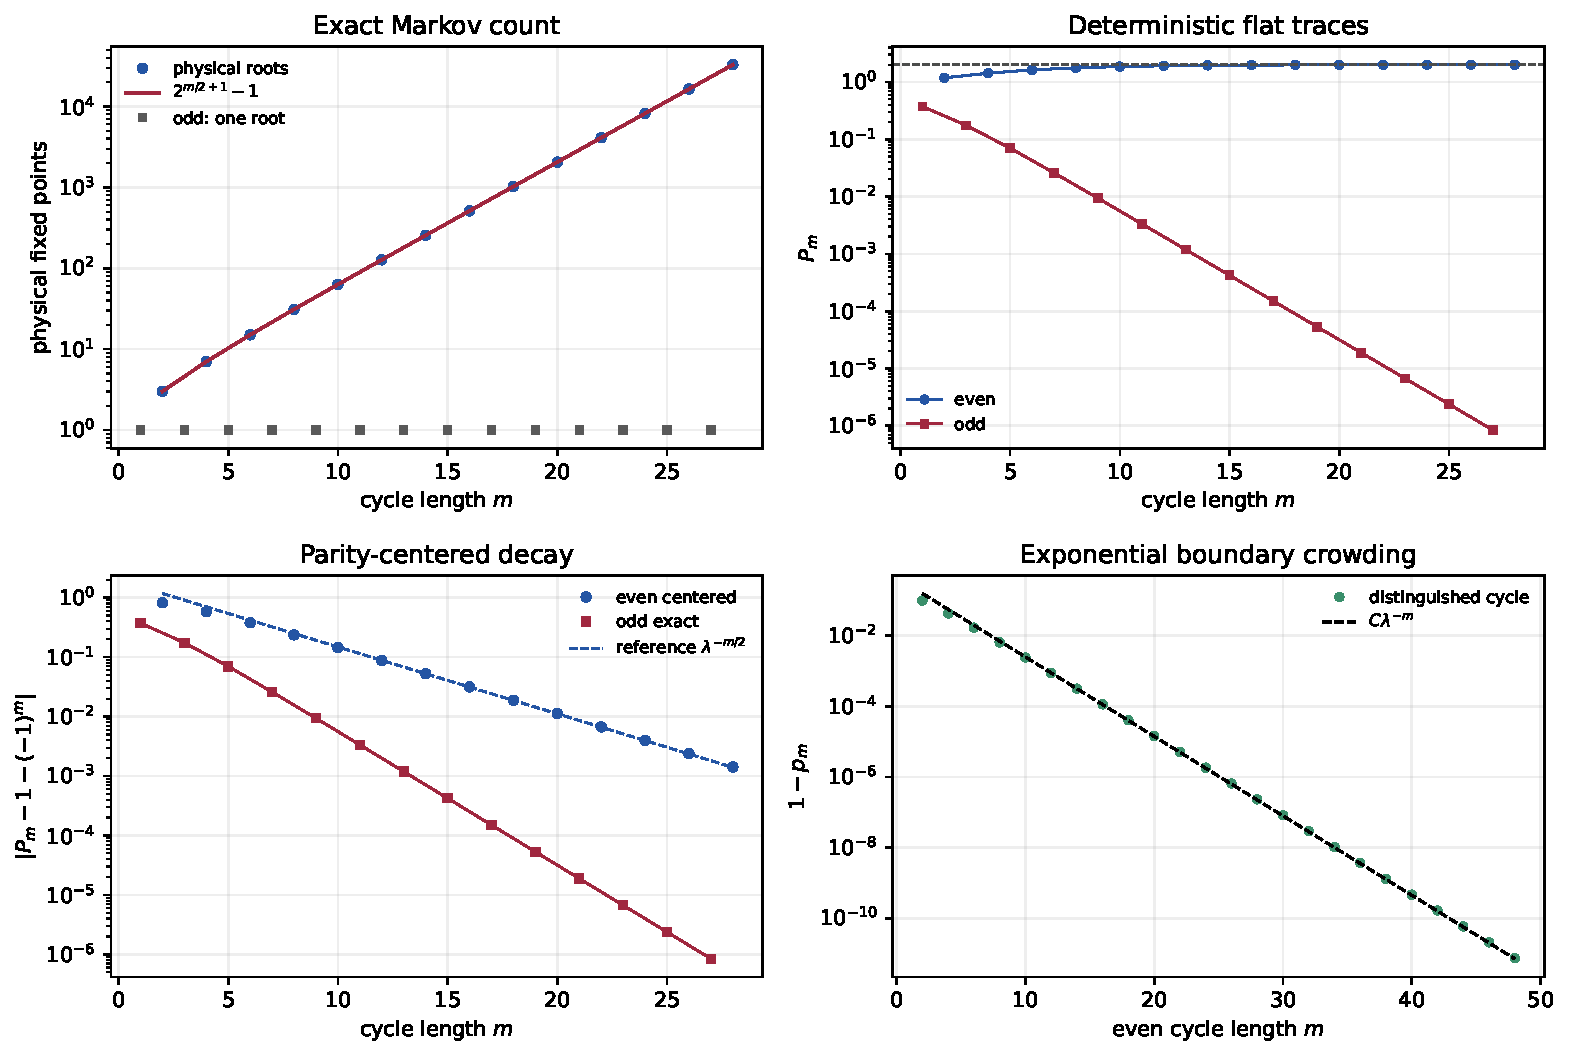
\includegraphics[width=\textwidth]{figures/deterministic_long_cycles.pdf}
\caption{Deterministic audit.  Top left: physical root counts lie exactly on
$2^{m/2+1}-1$ at even lengths, while every odd length has one boundary fixed
point.  Top right: odd traces decay and even traces approach the parity
baseline numerically.  Bottom left: parity-centered traces; the dashed even
rate is a numerical reference, not a theorem.  Bottom right: the explicitly
constructed boundary cycle follows $C\lambda^{-m}$.}
\label{fig:deterministic}
\end{figure}

\subsection{Negative resonance and two cycle scales}

At every tested noise level the folded matrix has a real negative resonance
separated from the remaining spectrum.  \Cref{tab:parity-resonance} records it
along with the bulk spectral radius after removing $1$ and $\lambda_-$.  A log--log
fit over the five smallest noise levels gives
\begin{equation}\label{eq:two-thirds-fit}
 1+\lambda_-(\sigma)
 \simeq0.2881505\,\sigma^{0.6674161}.
\end{equation}
The scaled gap is nearly constant over the tail.  At $\sigma=0.01$, increasing
$n$ from $1024$ to $2560$ changes $\lambda_-$ by
$2.34\times10^{-5}$, which is $0.17\%$ of the measured gap.

\begin{table}[t]
\centering
\small
\caption{Resolved negative parity resonance.  The $2/3$ scaling is numerical
evidence.  The bulk radius removes both the Perron and negative modes.}
\label{tab:parity-resonance}
\begin{tabular}{rrrrr}
\toprule
$\sigma$ & $n$ & $\lambda_-$ & $(1+\lambda_-)/\sigma^{2/3}$ & bulk radius\\
\midrule
0.080 & 256  & $-0.93736537$ & 0.33736 & 0.46206\\
0.060 & 342  & $-0.95194498$ & 0.31355 & 0.56193\\
0.050 & 410  & $-0.95883854$ & 0.30328 & 0.58907\\
0.040 & 512  & $-0.96535455$ & 0.29621 & 0.57356\\
0.030 & 683  & $-0.97194943$ & 0.29053 & 0.55714\\
0.020 & 1024 & $-0.97909426$ & 0.28373 & 0.65643\\
0.015 & 1366 & $-0.98268143$ & 0.28474 & 0.68226\\
0.012 & 1707 & $-0.98492256$ & 0.28766 & 0.67713\\
0.010 & 2048 & $-0.98655340$ & 0.28970 & 0.67467\\
\bottomrule
\end{tabular}
\end{table}

If \eqref{eq:two-thirds-fit} persists, the parity e-folding scale is
\begin{equation}\label{eq:parity-lifetime}
 m_{\mathrm{par}}(\sigma)
 \asymp\frac{1}{1+\lambda_-(\sigma)}
 \asymp\sigma^{-2/3}.
\end{equation}
This is parametrically longer than the rigorous localization ceiling
\begin{equation}\label{eq:localization-scale}
 m_{\mathrm{loc}}(\sigma)
 \lesssim\frac{\log(1/\sigma)}{\log\lambda}.
\end{equation}
At $\sigma=0.01$, the two diagnostics are approximately $74.4$ and $8.9$.
Their separation explains why finite-noise traces can retain a long parity
transient even though the termwise deterministic orbit proof has already lost
uniform boundary control.

\Cref{tab:trace-return} illustrates the eventual fixed-noise limit.  The bulk
part becomes negligible by length $20$ at $\sigma=0.015$; the remaining slow
return is almost entirely $1+\lambda_-^m$.

\begin{table}[t]
\centering
\small
\caption{Trace decomposition at $\sigma=0.015$ and folded dimension $1366$.
The equality raw $=$ peripheral $+$ bulk holds to rounding.}
\label{tab:trace-return}
\begin{tabular}{rrrr}
\toprule
$m$ & $\tr K_\sigma^m$ & $1+\lambda_-^m$ & bulk trace\\
\midrule
2   & 1.18300258 & 1.96566279 & $-7.82660\times10^{-1}$\\
4   & 1.48409214 & 1.93250463 & $-4.48412\times10^{-1}$\\
6   & 2.21486409 & 1.90048503 & $ 3.14379\times10^{-1}$\\
20  & 1.70543195 & 1.70510693 & $ 3.25018\times10^{-4}$\\
100 & 1.17429098 & 1.17429098 & $ 4.90\times10^{-17}$\\
200 & 1.03037735 & 1.03037735 & $ 1.17\times10^{-33}$\\
\bottomrule
\end{tabular}
\end{table}

\begin{figure}[t]
\centering
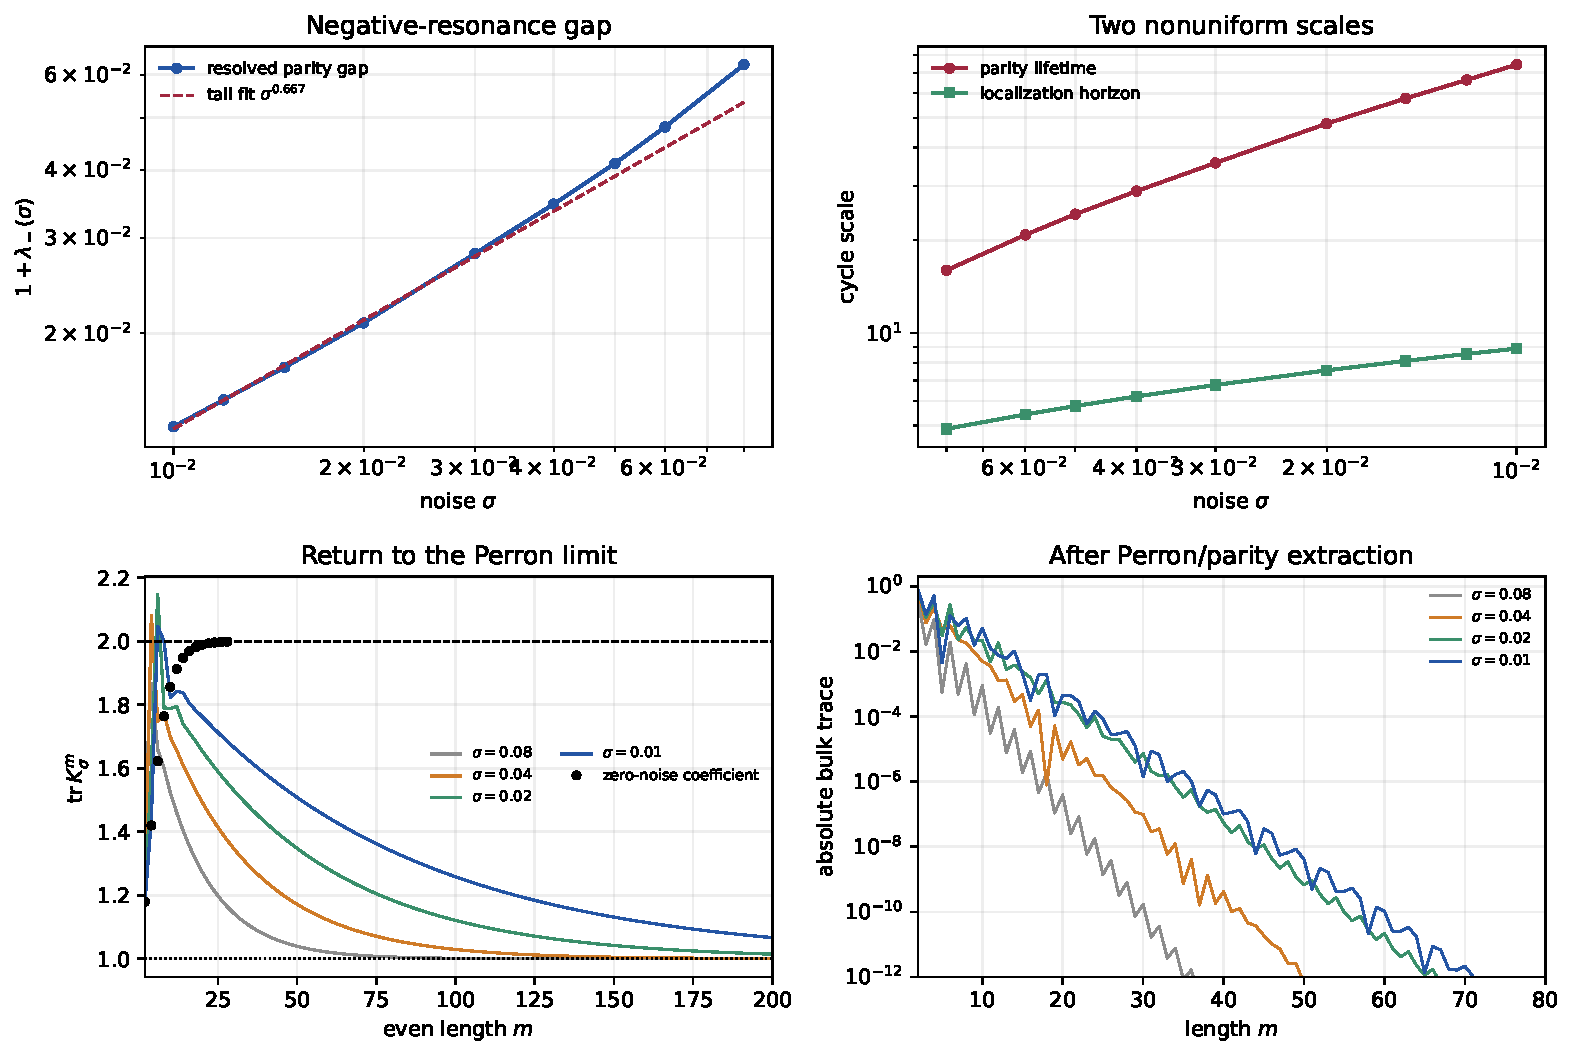
\includegraphics[width=\textwidth]{figures/noncommuting_long_cycle_limits.pdf}
\caption{Finite-noise long-cycle behavior.  Top left: the negative-resonance
gap and its five-point tail fit.  Top right: the numerical parity lifetime is
already much longer than the rigorous logarithmic localization horizon.
Bottom left: every fixed-noise even trace ultimately returns to $1$, while the
fixed-length zero-noise coefficients approach $2$ numerically.  Bottom right:
after extracting Perron and parity, the remaining traces decay rapidly.}
\label{fig:noncommuting}
\end{figure}

\subsection{Bulk determinant audit}

For each finite matrix, \eqref{eq:noisy-bulk-det-traces} truncated at
$m=120$ agrees with the direct eigenvalue product
\eqref{eq:noisy-bulk-det-product} to at worst
$2.51\times10^{-14}$ over all tested $z\in[0.25,1.10]$.  This verifies the
factorization independently of the deterministic comparison.

The deterministic curve in \cref{fig:determinants} is the explicit 28-term
centered trace truncation.  At $\sigma=0.01$, the finite-noise difference is
$0.00436$ at $z=0.5$, $0.10322$ at $z=0.9$, and $0.63235$ at $z=1.1$.
Approach is clear well inside the unit disk and progressively slower as $z$
weights longer cycles more strongly.  This is the expected signature of
coefficientwise convergence without a proved common long-cycle bound.

\begin{figure}[t]
\centering
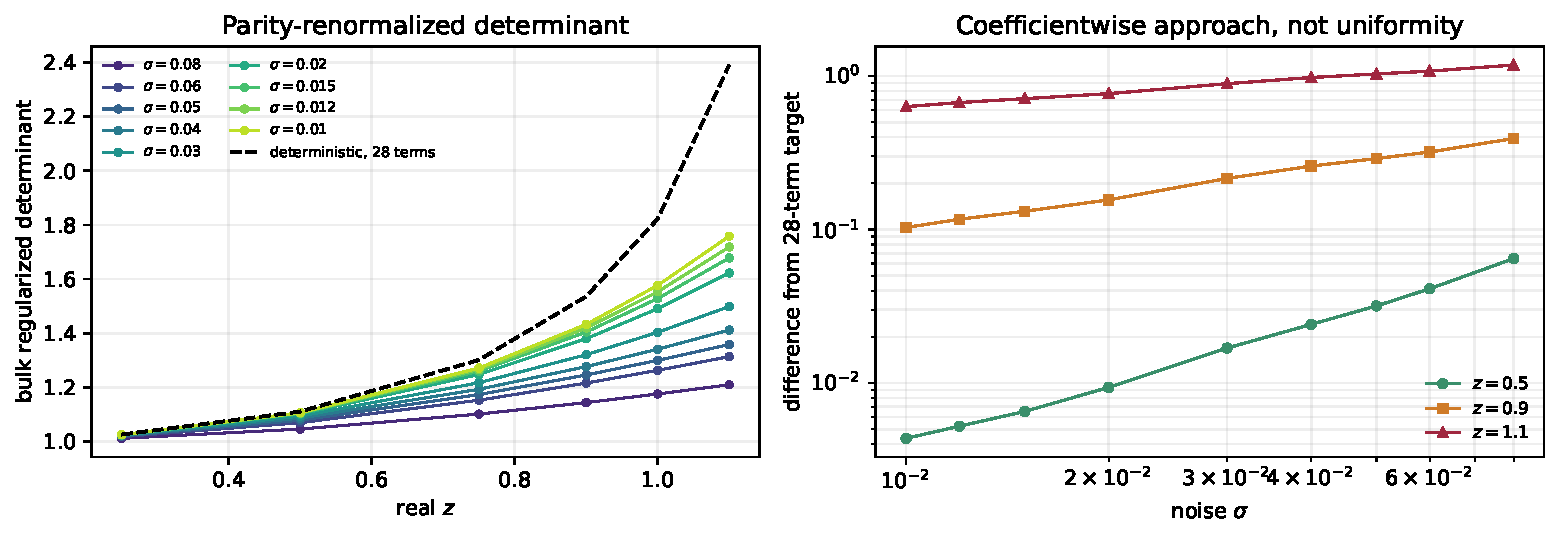
\includegraphics[width=\textwidth]{figures/bulk_determinants.pdf}
\caption{Parity-renormalized regularized determinants.  Left: finite-noise
bulk products approach the deterministic 28-term centered curve as the noise
decreases.  Right: the difference is small at $z=0.5$ but remains substantial
at $z=1.1$, where long coefficients receive greater weight.  The comparison
is between explicit truncations and is not claimed as uniform determinant
convergence.}
\label{fig:determinants}
\end{figure}

\FloatBarrier
\section{Discussion}
\label{sec:discussion}

The results resolve the first long-cycle question left open by the
fixed-length localization theorem.

First, the number of relevant deterministic saddles is known exactly.  The
factor $2^{m/2}$ comes from the bipartite Markov graph, while the physical
$-1$ correction comes from the double code of $r$.  This distinction is
topological and survives any numerical refinement.

Second, an explicit cycle reaches the integration boundary exponentially
fast.  Therefore a proof based on independent full-Gaussian neighborhoods of
every deterministic cycle cannot remain uniform for polynomially long
cycles.  The natural ceiling is logarithmic in $1/\sigma$.  This does not rule
out a boundary-layer determinant, but it specifies the new local model that
such a construction must contain.

Third, the raw long-cycle trace is the wrong object for comparing positive
noise with the deterministic limit.  Fixed noise has one permanent peripheral
mode; the deterministic map has two.  Removing the actual Perron and negative
resonances produces a bulk trace whose decay is visible both algebraically and
numerically.  The factor $1-z^2$ is not a fitted correction: it follows
exactly from the two parity coefficients.

Two analytic tasks remain separate.  One is deterministic: construct an
adapted flat-trace space and discharge \cref{ass:flat-trace-gap}.  The other
is stochastic: prove spectral stability of the negative resonance and derive,
or refute, the observed $2/3$ boundary-layer law.  Neither task is solved by
increasing matrix dimension alone.

\section{Conclusion}

At the quadratic band-merging parameter, long cycles expose a singular double
limit that fixed-length asymptotics cannot see.  Exact Markov coding gives the
physical periodic-point count and an exact odd trace formula.  Explicit
inverse branches produce a primitive cycle at distance
$\Theta(\lambda^{-m})$ from the boundary, forcing a logarithmic uniform
localization horizon.  Strong positivity at every fixed noise forces the
opposite long-time behavior, namely convergence of the trace to one.

Under one clearly isolated deterministic flat-trace hypothesis, these facts
prove that the small-noise and even long-cycle limits are $1$ and $2$ in
opposite orders.  The appropriate spectral object is consequently the
Perron/parity-renormalized Hilbert--Schmidt determinant.  Numerics support a
long-lived negative resonance with a $2/3$ gap law, but the manuscript keeps
that observation outside the theorem layer.  The next theoretical step is
therefore well posed: an adapted deterministic flat-trace construction and a
small-noise parity boundary-layer analysis, rather than an unqualified raw
determinant limit.

\section*{Data and code availability}

The source code, tests, machine-readable CSV and JSON results, and figure
generation script are available in the companion repository
\citep{WangLongCycleCode2026}.  The test suite verifies the algebraic orbit,
Markov spectrum, exact root counts, periodic residuals, odd trace identity,
boundary rate, stochasticity, spectral trace decomposition, and equality of
the regularized trace series with the eigenvalue product.

\bibliographystyle{unsrtnat}
\bibliography{references}

\end{document}
